\textit{Solución.} Se obtuvieron las siguientes respuestas para el sistema linealizado $H _{linealizado}(t)$ y el sistema real $H _{real}(t)$ ante los cambios especificados en el enunciado.

\begin{figure}[!h]
    \centering
    \begin{minipage}{0.5\linewidth}
        \centering
        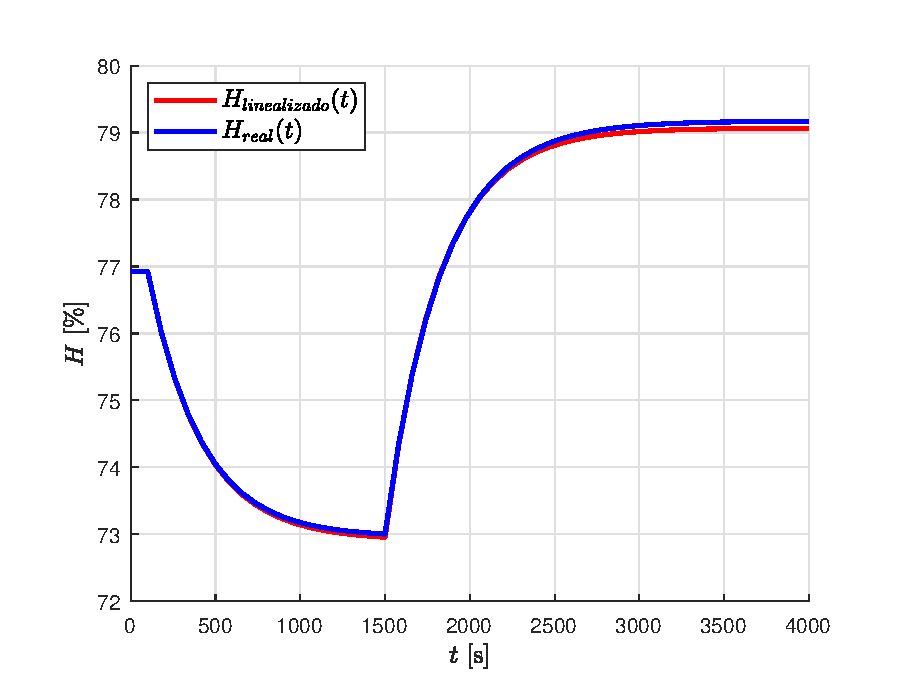
\includegraphics[width = 0.8\linewidth]{figs/fig4.eps}
        \caption*{(a): $\Delta U = -2\% \quad \Delta D = -0.02$}
    \end{minipage}%
    \begin{minipage}{0.5\linewidth}
        \centering
        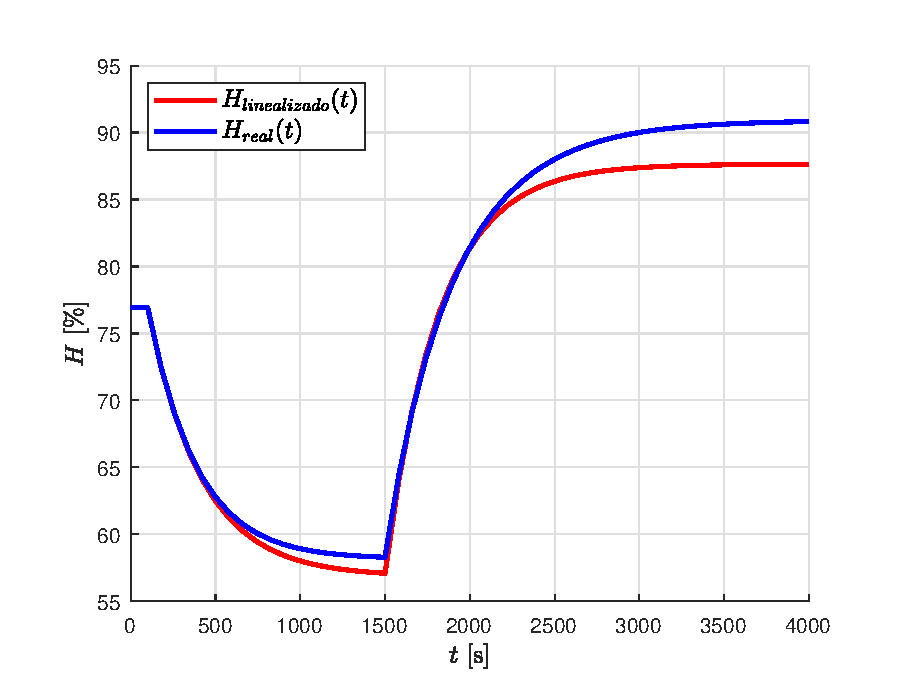
\includegraphics[width = 0.8\linewidth]{figs/fig5.eps}
        \caption*{(a): $\Delta U = -10\% \quad \Delta D = -0.1$}
    \end{minipage}
    \caption{Respuesta del sistema real y linealizado, ante distintas señales de control y perturbaciones.}
    \label{fig4}
\end{figure}
\newpage
